%########################################################
%
% Postprocessing LaTeX script
%
% Copyright: UW Computational Mechanics Group
%            Pedro Arduino
%
% Participants: Alborz Ghofrani
%               Long Chen
%
%-------------------------------------------------------

\documentclass[11pt,fleqn]{article}

\usepackage[T1]{fontenc}
\usepackage[ansinew]{inputenc}
\usepackage{fullpage, url}
\usepackage{amsmath, amsfonts}

\usepackage[normalem]{ulem}
\usepackage{longtable}
\usepackage{xcolor}
\usepackage{graphicx}
\newcommand\suppress[1]{}
\newcommand\deleted[1]{\xout{#1}}
\newcommand\revised[1]{\uline{#1}}
\newlength\wvtextpercent
\setlength\wvtextpercent{0.009\textwidth}

% \newif\ifpdf
% \ifx\pdfoutput\undefined
%   \pdffalse
% \else
%   \pdfoutput=1
%   \pdftrue
% \fi

%\ifpdf
%  \usepackage[pdftex]{xcolor}
%  \usepackage[pdftex]{graphicx}
%  \pdfinfo {
%    /Title (Materials Modeling)
%    /Subject (Transition from 1D to 3D)
%    /Author (Peter Mackenzie)
%    /Keywords (CEE503)
%  }
%\else
%  \usepackage{xcolor}
%  \usepackage{graphicx}
%\fi

\setlength{\parindent}{0pt}
\setlength{\parskip}{1ex plus 0.5ex minus 0.2ex}

\input{short}
\input{macros}


\begin{document}

%\tableofcontents
%\newpage
	\begin{center}
	
		\textbf{{DesignSafe Example\hfill{}1D Site Response Examples\hfill{}May 2017}}

	\end{center}
   

\section{Soil profile}

Free field response of single soil profile subjected to earthquake excitation

\begin{figure}[h!]
\centering
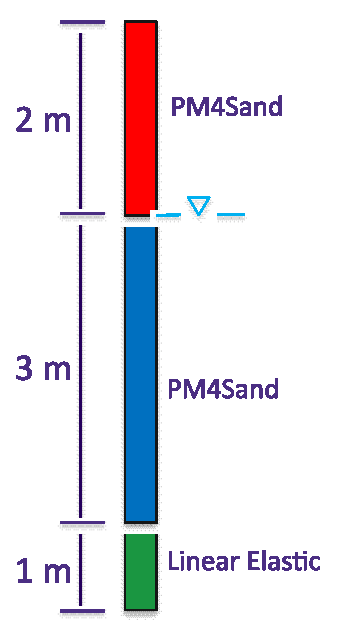
\includegraphics[scale=0.7]{schematic}
\caption{1D Model}
\end{figure}

\newpage
\section{Results}

% Plot Results
\begin{figure}[h!]
\centering
\includegraphics[width=5in]{surfaceAccel}
\caption{Surface acceleration time history}
\end{figure}

\begin{figure}[h!]
\centering
\includegraphics[width=5in]{logSpectra}
\caption{Surface response spectra}
\end{figure}



\end{document}
